% ================================================================
% INTRODUCTION
% ================================================================

\chapter*{Introduction}

TOP (Tracers in the Ocean Paradigm) handles oceanic passive tracers in NEMO. At present, this component provides the physical constraints and boundaries conditions for oceanic tracers transport and represents a generalized, hardwired interface toward biogeochemical models to enable a seamless coupling.

It includes three independent components :

\begin{itemize}
        \item a transport code TRP sharing the same advection/diffusion routines with the dynamics, with specific treatment of some features like the surface boundary
conditions, or the positivity of passive tracers concentrations
        \item sources and sinks - SMS - models that can be typically biogeochemical, biological or radioactive
        \item an offline option which is a simplified OPA 9 model using fields of physics variables that are previously stored to disk
\end{itemize}

There is two ways of coupling TOP to the dynamics :

\begin{itemize}
        \item \textit{online coupling} : the evolution of passive tracers is computed along with the dynamics
        \item \textit{offline coupling} : the fields of physics variables are read from files and interpolated at each model time step, with no constraints on the time sampling in the input files
\end{itemize}

TOP is designed to handle multiple oceanic tracers through a modular approach and it includes different sub-modules :

\begin{itemize}
        \item the ocean water age module (AGE) tracks down the time-dependent spread of surface waters into the ocean interior
        \item inorganic carbon (e.g. CFCs, SF6) and radiocarbon (C14) passive tracers can be modeled to assess ocean absorption timescales of anthropogenic emissions and further address water masses ventilation
        \item a built-in biogeochemical model (PISCES) to simulate lower trophic levels ecosystem dynamics in the global ocean
        \item a prototype tracer module (MY\_TRC) to enable user-defined cases or the coupling with alternative biogeochemical models ( e.g. BFM, MEDUSA, ERSEM, BFM, ECO3M)
\end{itemize}

\begin{figure}[ht]
\begin{center}
\vspace{0cm}
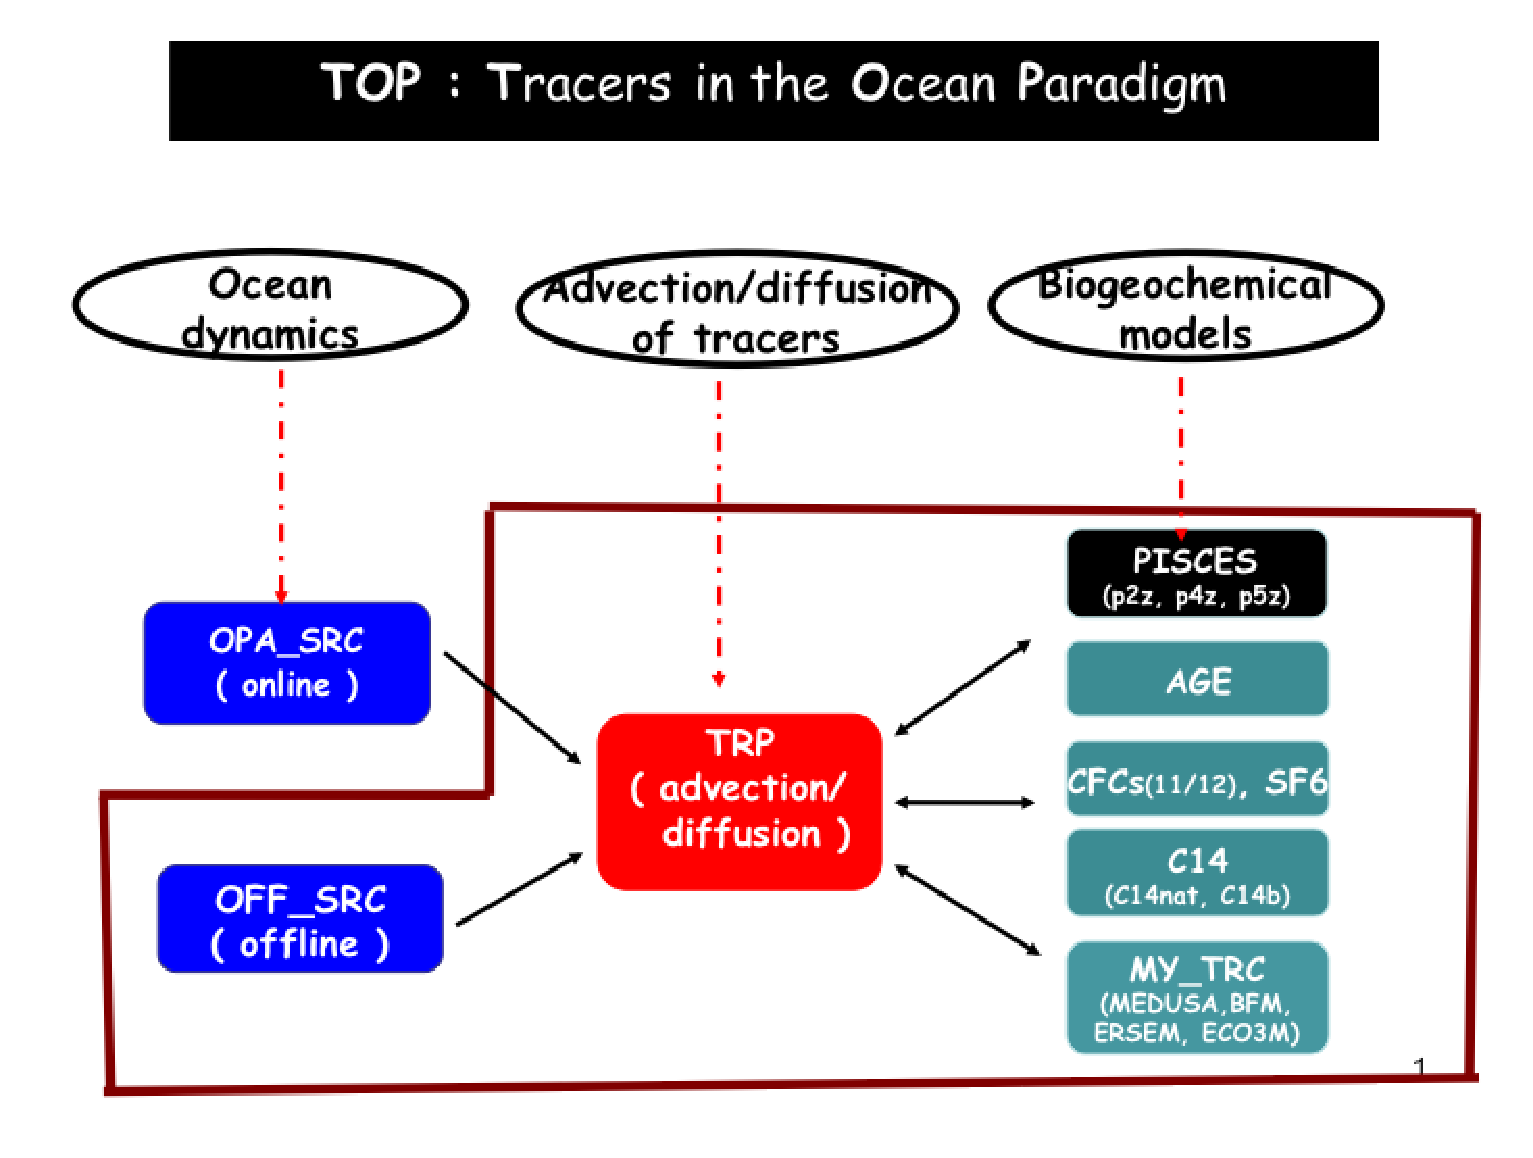
\includegraphics[width=0.80\textwidth]{Fig_TOP_design}
%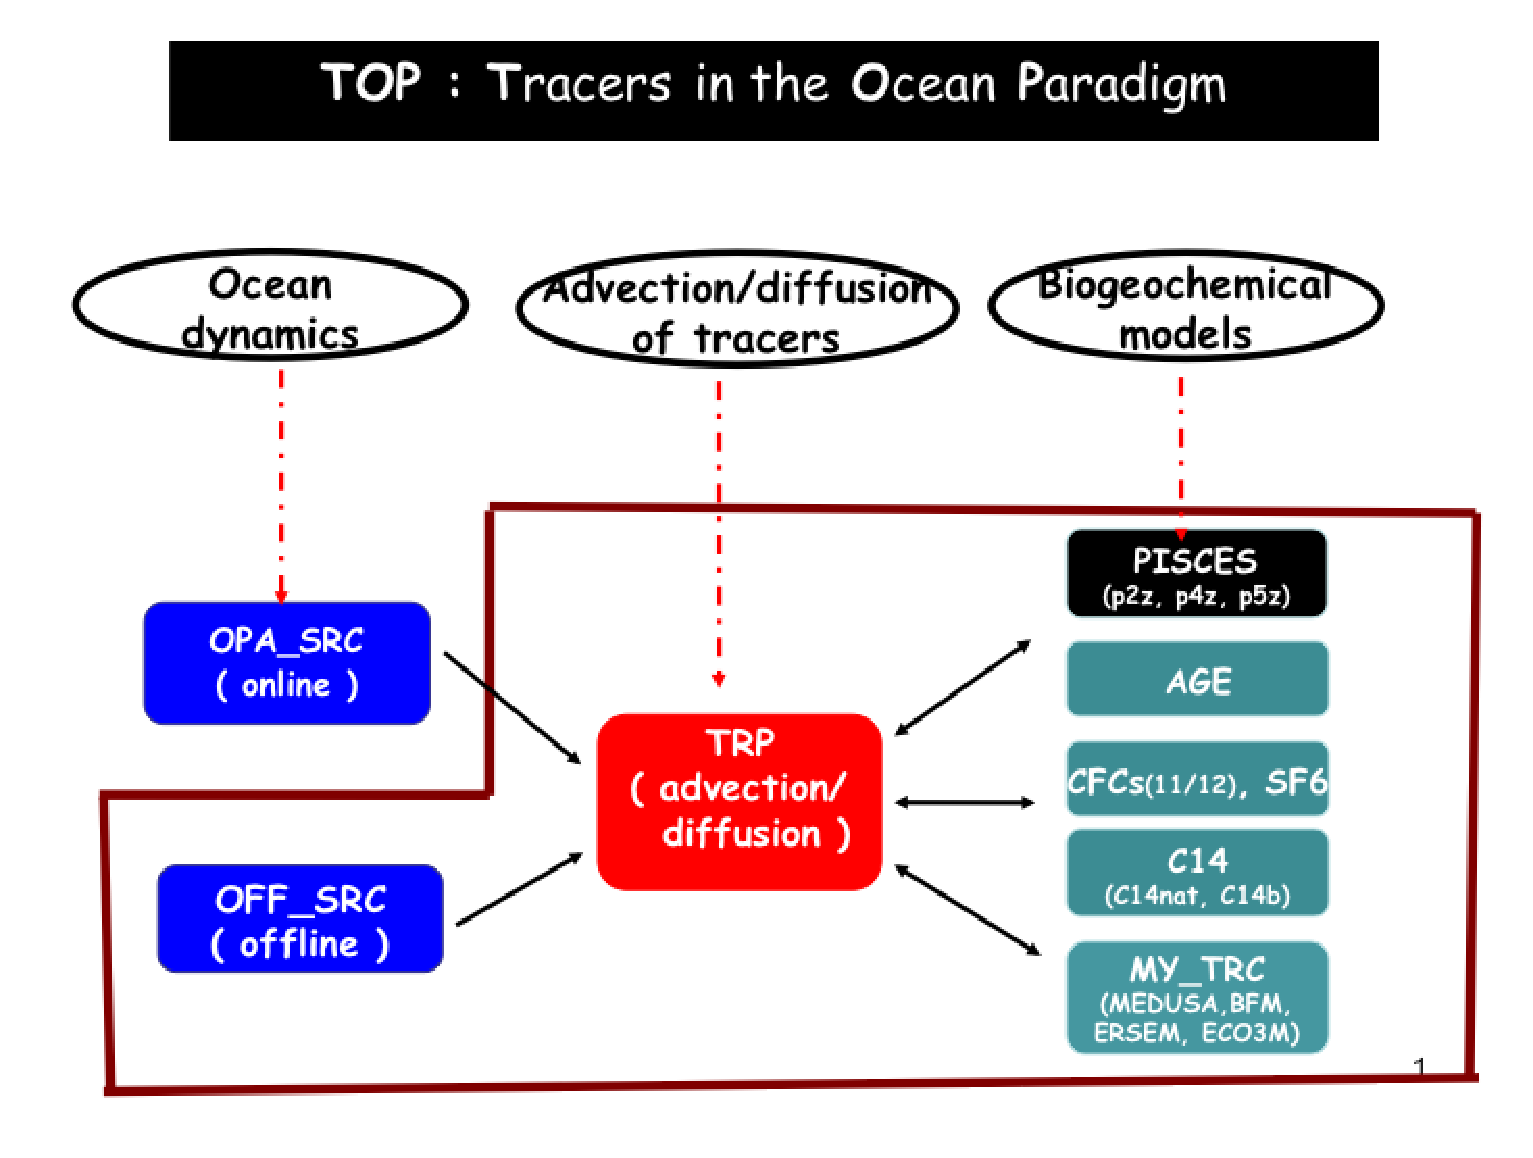
\includegraphics[height=6cm,angle=-00]{Fig_TOP_design}
\caption{A schematic view of NEMO-TOP component}
\label{topdesign}
\end{center}
\end{figure}
